% Part III-C, results of the tree GRPO runs (included by main_en.tex).
% DRAFT, written with seed 1 of both tree conditions; every claim is to be checked against both seeds and rlvr's three.

\section{Training with tree rollouts}\label{sec:res-tree}

Both tree conditions ran with \NUM{seeds_treekev} seeds of 200 steps, everything else as in Part II's \texttt{rlvr},
which is the flat reference (\NUM{seeds_rlvr} seeds). Table~\ref{tab:tree-acc} gives the final policies' accuracies,
Table~\ref{tab:tree-paired} the paired differences, Table~\ref{tab:tree-stats} what happened inside the trees during
training, and Figure~\ref{fig:tree-curves} the training curves. The intervals resample problems and do not include the
variation between seeds.

\paragraph{The judge's choice gained little over a random one.} Every tenth step the roots that were not kept are
continued too, so we know what keeping the chosen two gained over keeping all four (Table~\ref{tab:tree-stats}). Under
\texttt{tree\_kev} the leaves of the two roots \kev{} ranked highest were correct \NUM{auditgain_all_treekev}
\ci{\NUM{auditgainlo_all_treekev}}{\NUM{auditgainhi_all_treekev}} points more often than the leaves of all four roots,
over \NUM{auditgain_records_treekev} audited steps. Under \texttt{tree\_random}, whose choice gains nothing in
expectation, the same number is \NUM{auditgain_all_treerand}
\ci{\NUM{auditgainlo_all_treerand}}{\NUM{auditgainhi_all_treerand}}; these intervals resample the audited steps.
Keeping the two roots whose leaves turned out best would have gained \NUM{auditbest_all_treekev} points, more than any
ranking made before the leaves exist could, since the same four leaves per root both rank the roots and score them. On
the audited steps \kev{}'s \emph{on track} score of a root separates its correct from its incorrect leaves with an AUROC
of \NUM{auditotauc_all_treekev} pooled over prompts, but only \NUM{auditotaucw_all_treekev}
\ci{\NUM{auditotaucwlo_all_treekev}}{\NUM{auditotaucwhi_all_treekev}} within a prompt, the comparison that decides which
roots are kept (\NUM{auditotaucw_all_treerand} under \texttt{tree\_random}). Offline, with the same structure (four
prefixes of 128 tokens per problem, four continuations each), the within-problem AUROC was \NUM{aucw_128_kevtrack}, and
keeping the two best-ranked prefixes raised the share of continuations ending correct by \NUM{gainpt_128_kevtrack}
points (\S\ref{sec:res-prefix}). The prefixes differ: offline they are the base policy's, in training the policy's own
as it learns. Its roots lead to correct answers more and more often (under \texttt{tree\_random},
\NUM{auditval_firsthalf_treerand}\% of the audited leaves were correct in the first half of training and
\NUM{auditval_secondhalf_treerand}\% in the second, against a mean value of \NUM{ps_valueall_128} for the base policy's
prefixes offline), and the room for a choice, the best two in hindsight, shrank from \NUM{auditbest_firsthalf_treerand}
to \NUM{auditbest_secondhalf_treerand} points.

\begin{table}[t]
\centering\small
\begin{tabular}{@{}lcccccccc@{}}
\toprule
 & & roots & \multicolumn{5}{c}{audit, every 10th step: all four roots continued} & tokens \\ \cmidrule(lr){4-8}
condition & seeds & ended & AUROC & within prompt & value & gain, kept 2 & gain, best 2 & per step (k) \\ \midrule
\texttt{tree\_random} & 3 & 1.5\% & 0.75 & 0.56 & 60.6 & $+$0.3 & $+$8.1 & 65.1 \\
\texttt{tree\_kev} & 3 & 1.3\% & 0.75 & 0.55 & 59.9 & $+$1.4 & $+$8.4 & 74.7 \\
\bottomrule
\end{tabular}

\caption{Inside the trees during training (mean over steps and seeds): share of roots that had already ended within 128
tokens; on the audited steps (every tenth), where all four roots of a prompt are continued, the AUROC of \kev{}'s
\emph{on track} score of a root for its leaves' verdicts, pooled and within prompt, the leaf accuracy of all four roots
(percent), and what keeping the chosen two, or the best two in hindsight, gained over it (points); tokens generated per
step (thousands, last 20 steps), not counting the audit's continuations.}
\label{tab:tree-stats}
\end{table}

% TODO after seed 2: final accuracies; tree_kev against tree_random (selection) and tree_random against rlvr (tree
% shape), at step 200 and at step 100; whether the seed-1 gap of tree_kev survives.
\paragraph{Final accuracy.} Table~\ref{tab:tree-acc}.

\begin{table}[t]
\centering\small
\begin{tabular}{@{}lcccccc@{}}
\toprule
condition & seeds & MATH-500 & GSM8K & AMC23 & AIME24 & AIME25 \\ \midrule
base model & -- & 76.5 & 87.9 & 50.6 & 10.0 & 10.9 \\ \midrule
\texttt{rlvr} & 2 & 82.9 $\pm$ 0.1 & 93.2 $\pm$ 0.2 & 61.7 $\pm$ 2.7 & 21.5 $\pm$ 0.6 & 17.8 $\pm$ 1.3 \\
\texttt{tree\_random} & 2 & 84.5 $\pm$ 3.0 & 93.1 $\pm$ 1.0 & 67.0 $\pm$ 5.0 & 27.2 $\pm$ 8.7 & 20.5 $\pm$ 6.0 \\
\texttt{tree\_kev} & 2 & 84.9 $\pm$ 3.3 & 94.1 $\pm$ 0.9 & 65.8 $\pm$ 3.8 & 26.4 $\pm$ 7.8 & 20.0 $\pm$ 6.2 \\
\bottomrule
\end{tabular}

\caption{Final policies: accuracy in percent, seed mean $\pm$ standard deviation over seeds. MATH-500 and GSM8K: greedy.
AMC23, AIME24 and AIME25: mean over 16 samples per problem at temperature 0.6. \texttt{rlvr}: flat sampling (Part II).}
\label{tab:tree-acc}
\end{table}

\begin{table}[t]
\centering\small
\begin{tabular}{@{}lccccc@{}}
\toprule
minus \texttt{tree\_random} & MATH-500 & GSM8K & AMC23 & AIME24 & AIME25 \\ \midrule
\texttt{rlvr} & $-$1.6 & $+$0.1 & $-$5.2 & $-$5.7 & $-$2.7 \\
 & {\footnotesize \ci{$-$3.6}{0.3}} & {\footnotesize \ci{$-$0.8}{0.9}} & {\footnotesize \ci{$-$9.3}{$-$1.6}} & {\footnotesize \ci{$-$10.3}{$-$1.5}} & {\footnotesize \ci{$-$5.7}{0.1}} \\[2pt]
\texttt{tree\_kev} & $+$0.4 & $+$1.0 & $-$1.2 & $-$0.8 & $-$0.5 \\
 & {\footnotesize \ci{$-$1.6}{2.3}} & {\footnotesize \ci{0.2}{1.9}} & {\footnotesize \ci{$-$3.4}{1.0}} & {\footnotesize \ci{$-$3.5}{1.6}} & {\footnotesize \ci{$-$3.5}{2.6}} \\[2pt]
\bottomrule
\end{tabular}

\caption{Paired differences to \texttt{tree\_random} in percentage points: per problem, each condition's seed mean,
averaged over problems, with a 95\% bootstrap interval over problems. \texttt{tree\_kev} minus \texttt{tree\_random}
isolates the judge's choice of roots; \texttt{rlvr} minus \texttt{tree\_random} the tree shape.}
\label{tab:tree-paired}
\end{table}

\paragraph{Cost.} A tree generates every root, kept or not, and the continuations of the kept ones:
\NUM{gentok_treekev} thousand tokens per step under \texttt{tree\_kev} and \NUM{gentok_treerand} thousand under
\texttt{tree\_random}, against \NUM{gentok_rlvr} thousand for flat sampling (the last 20 steps). Scoring the roots with
\kev{} on the shared backbone is the only extra cost of the judge's choice.

\begin{figure}[t]
\centering
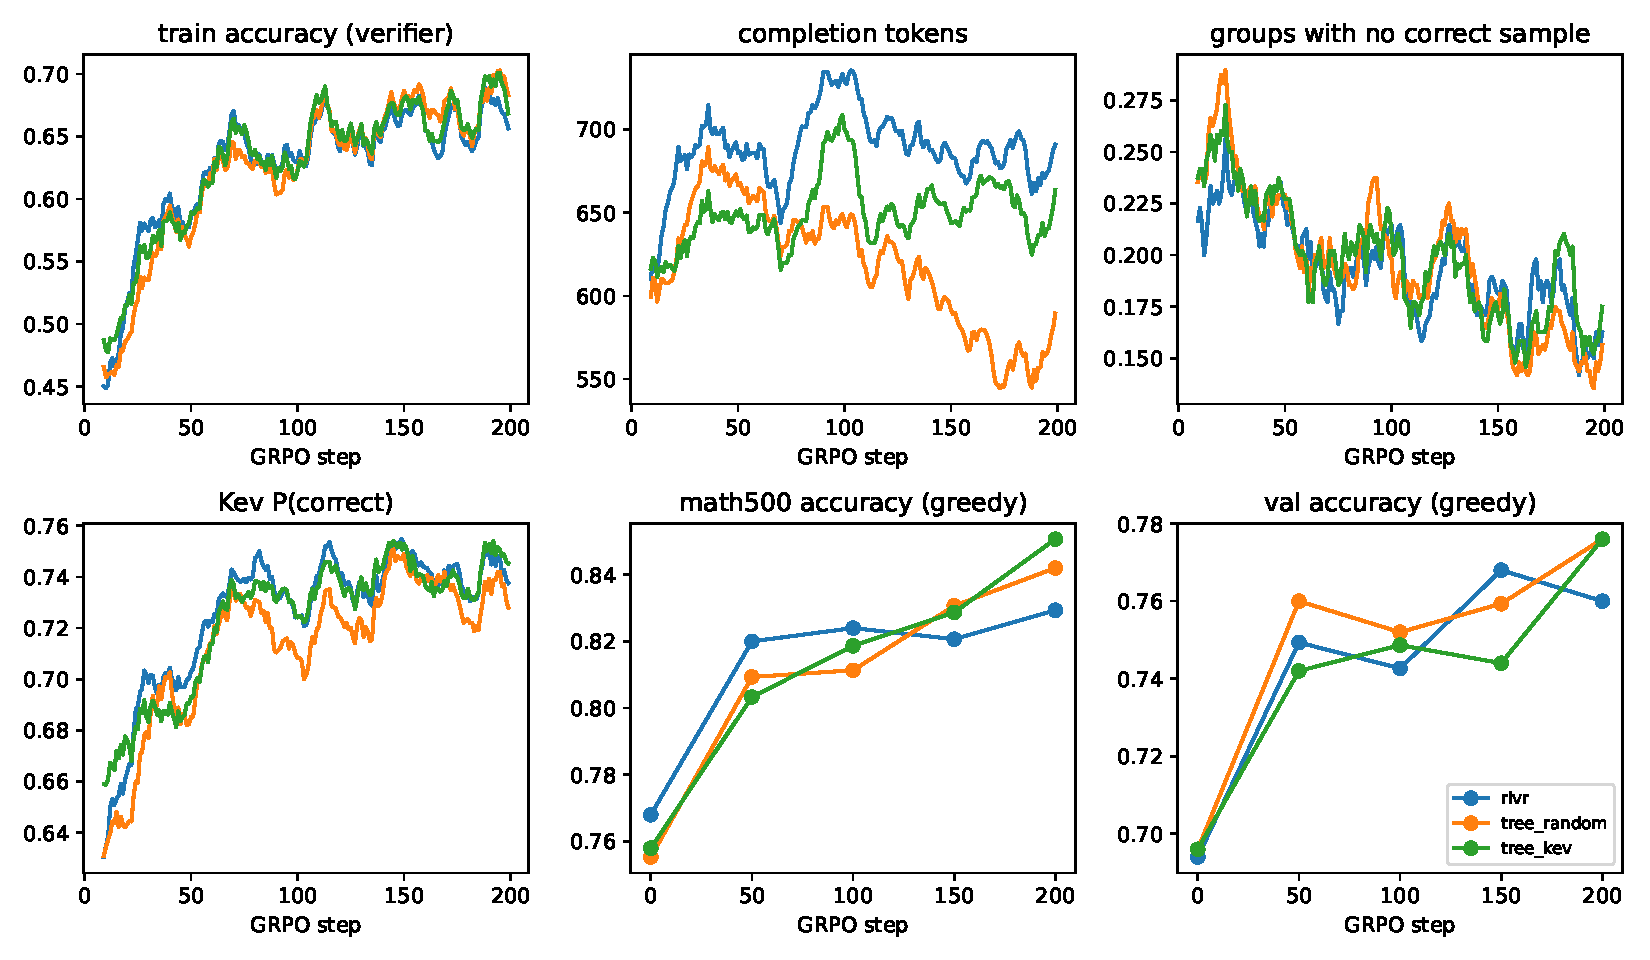
\includegraphics[width=\linewidth]{../../experiments/part3c_tree/results/training_curves.pdf}
\caption{Training curves (seed mean): verifier accuracy, completion tokens, share of groups with no correct completion
and \kev{}'s $\pc$ on the training completions (10-step moving averages), and greedy accuracy on MATH-500 and the
validation set every 50 steps.}
\label{fig:tree-curves}
\end{figure}

\paragraph{Evaluation noise.} Across the \NUM{szruns_math500} runs in this comparison, the base model's MATH-500
accuracy at step 0 ranges from \NUM{szmin_math500}\% to \NUM{szmax_math500}\%, and a run's accuracy changes by
\NUM{lecabs_math500} points on average between its evaluations at steps 150 and 200.
